\documentclass{article}
\usepackage{blindtext}
\usepackage{titlesec}
\usepackage[utf8]{inputenc}
\usepackage[parfill]{parskip}
\usepackage{algorithm}
\usepackage{algorithmic}
\usepackage{graphicx}

\usepackage{sectsty}

\usepackage{hyperref}

\begin{document}
\begin{titlepage}
    \begin{center}
        \vspace*{1cm}
        \Huge
        \textbf{Quantum particles in fractal external potential}

        \vspace{0.5cm}
        \Large
        Memory of the project
        \vfill
        \begin{figure}[h!]
            
\includegraphics[width=\textwidth]{./logo-fib.png}
        \end{figure}
        \textbf{Marc Amorós}\\
        \vspace{0.5cm}
        \textbf{Thesis supervisor: Grigori Astrakharchik}\\
        \vspace{0.5cm}

   \end{center}
\end{titlepage}

\tableofcontents
\break

\section{Context}

\subsection{Introduction}
The investigation world is always closely related to computer science. It is very frequent 
to solve a problem by modelling it on a computer using a certain programming language, and 
then making simulations to get a solution.\\

The physics investigation field highly benefits of this problem-solving approaches, as we 
find plenty of equations with physical meaning without an exact solution. To fix this, we 
try to solve them by representing these equations in a discrete and finite space, so our computers 
can handle it, and then we write algorithms to get approximations of a real solution.\\

This is an interdisciplinary research project, with an important theoretical part that involves 
some quantum physics knowledge and a practical part that covers the design and development of 
algorithms to simulate and solve quantum physics systems.\\

\subsection{Stakeholders}
It is important to define the stakeholders of any project, to know who is interested of its 
development and can benefit from it.\\

The main stakeholder of this project is UPC physics department, and more concretely Grigori 
Astrakharchikm, who was the impeller of it, by posting a TFG offer on Racó. This can lead to 
a scientific publication if interesting results are obtained, that is why it can interest him 
as a researcher.\\

As every scientific research project, it increases the knowledge on this field in general. If 
we write a paper about the steps we followed it can be beneficial for any other researcher of 
quantum particle systems and their unique properties, even they could try to replicate our 
results by real experimentation. So it can be considered that this project benefits all the 
scientific community in a way, more specifically the physics investigators.  


\subsection{Theoretical concepts}
I will summarize some theoretical concepts that are necessary to understand the rest of this 
document, so the reader can fully comprehend the aim and objectives of this project.

\subsubsection{Quantum mechanics}
Quantum mechanics is the theory that describes the physical properties of Nature at the scale 
of atoms and subatomic particles. When it was first formulated during the early decades of the 
20th century, it introduced some ground-breaking concepts, such as energy quantization, the 
uncertainty of position and momentum of a particle and the wave-particle duality of matter.\\

In classical physics we have Newton’s second law, which given a set of initial conditions 
makes a mathematical prediction of what path a given physical system will take over time. 
Its quantum analogous would be the Schrödinger equation, which instead requires a statistical 
interpretation.

\subsubsection{Schrödinger equation}
Quantum mechanics tells us how the particles behave over time. This description is done using 
the Schrödinger equation, which provides the time evolution of the wavefunction of particles.
The wavefunction, generally represented with the letter $\Psi$, is a mathematical 
description of the quantum state of the system, and with it, you can obtain the distribution
of probability of the measurements that you can do over this system.\\

The Schrödinger equation is a differential equation, and has the following form:


\begin{equation}
i\hbar\frac{\partial}{\partial t}\Psi\left(r,t\right)=\hat{H}\Psi\left(r,t\right)
\end{equation}
Here we define the Hamiltonian operator $\hat{H}$, which is an operator corresponding to the total energy of that system, including both kinetic ($T$) and potential energy ($V$), and for a single particle it takes the form:
\begin{equation}
\hat{H}=\hat{T}+\hat{V}=-\frac{\hbar^2}{2m}\nabla^2+V\left(r,t\right)
\end{equation}
The kinetic energy in quantum mechanics is proportional to the Laplace operator $\nabla^2$, which is the addition of the second partial derivatives of the wavefunction. The potential energy is a function of the position of the particle, similarly to the classical case.\\

We are interested in the stationary properties, so we take the time-independent version of the Schrödinger equation:
\begin{equation}
\hat {H} |\Psi \rangle = E |\Psi \rangle
\end{equation}
When solving it, the set of energy eigenvalues that provides (also called energy spectrum) is the set of possible energies obtained when measuring the system’s total energy. Here we are interested in finding the ground state of the system, which is its lowest energy state. Differently from the classical systems where the energy of a single particle at zero temperature is finite due to zero-point motion, this ground state energy is always present in the quantum system, even in absolute zero temperature conditions. 

\subsubsection{Fractals}
A fractal is a subset of the Euclidean space that illustrates a property called self-similarity, which means that appears the same at different scales and exhibits similar patterns at increasingly smaller scales. 

\subsubsection{Sierpiński carpet}
The Sierpiński carpet is a plane fractal that was first described by Wacław Sierpiński in 1916, as a two dimensions generalization of the Cantor set, that was discovered in 1874 by Henry John Stephen Smith and introduced by German mathematician Georg Cantor in 1883.\\

The Cantor ternary set is created by iteratively deleting the open middle third from a set of line segments.

\begin{figure}[h]
    
\includegraphics[width=\textwidth]{./cantor.png}
    \caption{First six steps of Cantor ternary set}
\end{figure}

To describe fractals properties we frequently use the fractal dimension, which is a ratio that 
provides a statistical index that shows how the detail in the pattern of the fractal changes
with every iteration. These leaves us with non integer dimensions, as the dimension of the 
Sierpiński carpet is $ log(8)/log(3)\approx 1,8927...$
\begin{figure}[h]
    \centering
    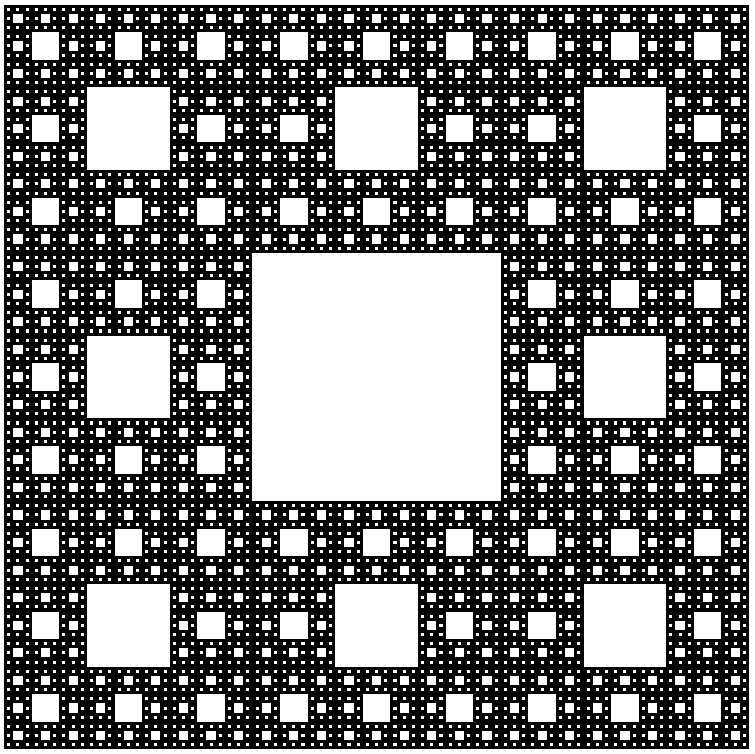
\includegraphics[scale=0.4]{./sierpinski.png}
    \caption{Sierpiński carpet with 5 levels of recursion}
\end{figure}
\vfill

\section{Justification}
The interdisciplinary aspect of this project is what attracts me the most. Quantum mechanics
is a complicated field that we do not study on the GEI degree. That is why this project 
really interested me personally, as it gives me the opportunity to learn and work on a 
subject that is quite different to what I am used to, and I am also able to contribute 
on a physics research project applying my computation knowledge, something I would enjoy
doing as a future job.\\

There have been recent experiments \cite{boseeinstein} that have shown how it is possible 
to produce a Bose-Einstein condensate. In the last few years, new experimental techniques 
have been developed, and it became feasible to create two-dimensional Fermi or Bose gas 
in highly controllable external potential. The projected potential can be chosen essentially 
in any desired shape, fractal shapes included. These means that most of our work could be 
verified by these experiments. Moreover, we could find some related articles that studied
the properties of particles on a fractal environment, but they did not obtain the energetic, 
structural and dynamic properties as we do.

\section{Objectives}
The aim of the project is to study the properties of quantum particles in a fractal external 
potential. The main goal is to obtain a detailed description of such a system in terms of 
energetic, structural and dynamic properties. In particular, the energetic properties can 
be quantified by evaluation of the ground state energy and the excitation spectrum. The 
structural property of interest is the density profile. The dynamic property to be calculated
is the diffusion coefficient.\\

We consider the external potential in the shape of a Sierpiński carpet. It has a fractal 
structure with the fractal dimensionality between 1 (i.e. a line) and 2 (i.e. a plane). 
The strength of the external potential is considered to be infinite (i.e. hard walls) in 
the positions where the fractal is present. It means that the particles cannot diffuse 
freely in the system. At the same time, the phase space is joined, that is the particle is 
allowed to move between any two points where the external field is absent. The fractal shape 
is defined in a simple recursive procedure and depends on the recursion level.\\

One of our goals is to provide a detailed description of the properties of quantum particles 
in fractal external potential. In particular, we plan to verify the existence of a simple 
scaling law between the recursion number of the zero-point energy of the system and the 
number of iterations of the fractal.\\

This is an interdisciplinary problem, based on application of mathematical concepts to the 
field of quantum physics, and relies on the use of numerical methods. This project requires 
carrying out a scientific investigation and a priori it is not clear which quantum system 
is going to be the best to study these properties.

\section{Scope}
We plan to execute this study considering three different problems:

\begin{enumerate}
    \item Solve Schrödinger equation using exact diagonalization of a discretized Hamiltonian
    \item Solve the time-dependent Schrödinger equation using the previous problem
    \item Do random walks over the Sierpinski carpet to obtain the diffusion coefficient 
\end{enumerate}




\section{Potential obstacles and risks}
\section{How the project will be developed}
\subsection{Methodology and rigour}
\section{Project phases}


\section{Sustainability}
\subsection{Reflection}
I have been aware for years that computer science can have a negative and positive impact on people's lives, on the environment and on the world in general. That's why I try to always think about the ethic consequences of my actions and not waste resources both in my particular life and on any kind of project I am involved on. I find that society does not give the social and environmental sustainability of projects the importance it deserves. 

In any project it is important to perform a sustainability analysis considering three dimensions: economic, environmental and social. 

\subsection{Economic dimension}
The different aspects of the economic dimension of this project are:
\begin{itemize}
    \item This project has a really reduced budget, as the main developer is a student. 
    \item We have established some strategies to entirely organize this project online, so we do not need any kind of office, what could be and additional cost.
    \item We could analyze the need of the renting of the server for the entire duration of the project, but as this is a research project we are not sure about how long we are going to need it. If we finish earlier we can always stop paying it.
    
\end{itemize}

\subsection{Social dimension}
We state some aspects of the social dimensions as follows: 
\begin{itemize}
    \item If we end up with interesting results, it is very likely that this project evolves in a scientific publication. These means that it contributes to the scientific knowledge as it is a research field that has not been properly explored yet.
    \item Our work can lead to other people getting interested in the study of the behaviour of quantum particles in a different shaped external potentials.
    \item It can also demonstrate and show off how important and successful an interdisciplinary project can be, something really important in a bast range of fields.
    
\end{itemize}


\subsection{Ambiental dimension}
To end up with our sustainability analisis, we explore the abiental aspects of the project:
\begin{itemize}
    \item The resources used to develop this project are the ones stated previously, we do not extract or use any kind of natural resource. We also do not emit or produce anything harmful for the environment.
    \item We do not waste office supplies and we try to cut down to the minimum the amount of it that we use.
    \item The programs that we run on the server are really optimized, to save computation time, and with it, energy. 
\end{itemize}

\break
\section{Solving Schrödinger equation with fractal external potential}



\break
\addcontentsline{toc}{section}{References}
\begin{thebibliography}{9}

\bibitem{BEC}The Gross-Pitaevskii Equation and Bose-Einstein condensates, J. Rogel-Salazar - 10 January 2013.

\bibitem{boseeinstein} 
Exotic fifth state of matter made on the International Space Station, New Scientist, by Jonathan O’Callaghan - 11 June 2020.

\bibitem{} Dynamical symmetry and breathers in a two-dimensionalbose gas,
R. Saint-Jalm, P. Castilho, E. L. Cerf, B. Bakkali-Hassani, J.-L. Ville, S. Nascimbene,J. Beugnon and J. Dalibard, Phys. Rev.X 9, 021035 - 2019.

\bibitem{} Quantum transport in Sierpinski carpets,
Edo van Veen, Shengjun Yuan, Mikhail I. Katsnelson, Marco Polini, and Andrea Tomadin
Phys. Rev. B 93, 115428 – 21 March 2016.

\bibitem{} Solving Hydrogen atom numerically with 14 lines of Matlab code 
[https://timqian.com/2015/03/04/H-atom-numerical/] - 04 March 2015.

\bibitem{} Fundamental Algorithms in Computational Fluid Dynamics, Thomas H. Pulliam, David W. Zingg, doi:10.1007/978-3-319-05053-9 - 2014.

\bibitem{} Solution of BVPs in electrodynamics by stochastic methods, 2007 IEEE Applied Electromagnetics Conference (AEMC), R. Janaswamy, Kolkata, India, pp. 1-4, doi: 10.1109/AEMC.2007.4638046. - 2007.

\bibitem{hores}FIB-UPC, “Normativa del treball final de grau del grau en enginyeria informàtica de la FIB,” 2012. [Online]. Avaliable:  https://www.fib.upc.edu/sites/fib/files/documents/actes/normativatfg-gei\_document\_final.pdf

\bibitem{TR}Taules retributives del personal docent i investigador laboral Any 2020  [https://www.upc.edu/transparencia/ca/informacio-de-personal/sdg8\_2\_1\_retribuciones\_pdi\_2020-1.pdf]

\bibitem{TFG_docu}Normativa del treball final de grau del grau en Enginyeria Informàtica de la Facultat d’Informàtica de Barcelona [https://www.fib.upc.edu/sites/fib/files/documents/estudis/normativa-tfg-mencio-addicional-gei-br.pdf]

\bibitem{LG}Amazon - LG gram 14Z90N-V-AA78B [https://www.amazon.es/LG-gram-14Z90N-V-AA78B-Ordenador-ultraligero/dp/B0861W8D24/]


\end{thebibliography}






\end{document}
